%\newpage

%//------ Section 01 -------------------------------------------------------------------------------------------------
\chapter{Particle physics}
\label{sec:Section01-Intro}
%//-----------------------------------------------------------------------//

Particle physics can fairly be defined as the field of Physics dedicated to the study of fundamental particles and the interactions between them. The idea that matter is composed of elementary bricks is not contemporary, though; the philosophical foundations of this idea date back to the Hellenic epoch in the Ancient Greece (\upperRomannumeral{5}$^{\text{th}}$ century BC)\footnote{The fathers of the Atomism from the Ancient Greece, Leucippus and Democritus, thought that matter was made of both void and elementary, indivisible corpuscules: atoms.} \cite{pullmanAtomHistoryHuman1998}. With the advent of the scientific method, this concept resurface through the 19th and 20th centuries with, among the most notables, Dalton's atomic theory\footnote{Apart from the name, it does not share much with the philosophical reasoning from the Ancient Greece.} and the discovery of the electron by J.J Thomson \cite{thomsonXLCathodeRays1897}. Although the first known particle, the electron, was discovered in 1897, research on particle physics gained momentum in the 1950s, thanks to the development of the particle accelerators. These devices made possible to observe high-energy collisions of known particles under controlled laboratory conditions and revealed the existence of dozens of particles: discovery of the pion \cite{lattesProcessesInvolvingCharged1947} and kaon in 1947 \cite{rochesterdr.EvidenceExistenceNew1947}, followed by the ones of the \rmLambda in 1950 \cite{hopperEvidenceConcerningExistence1950}, the anti-proton in 1955 \cite{chamberlainObservationAntiprotons1955}, the electron and muon neutrinos in 1956 \cite{reinesNeutrino1956} and 1962 \cite{danbyObservationHighEnergyNeutrino1962} respectively, the \rmXi in 1964 \cite{barnesObservationHyperonStrangeness1964}, etc. In total, more than 30 new particles were found by the early 1960s \cite{serwayModernPhysics2004} and it was still increasing. This particle "zoo" confused physicists for a decade. It is not until the 1970s that, thanks to the interplay between theory and experiment, a model successfully provided a unified description of these hundreds of particles: the latters are, in fact, composite objects, made of smaller and fewer constituents. This model still represents the best description of the sub-atomic universe to this day, hence its well-deserved name: the Standard Model of particle physics. The achievement of the Standard Model is a turning point in the history of Physics and marked the advent of modern particle physics.

\section{The Standard Model of particle physics}
\label{sec:StdModel}

\subsection{Theoretical aspects}
\label{subsec:Theory}

Mathematically speaking, the Standard Model is a (relativistic) quantum field theory (QFT), whose dynamics and kinematics are typically described by a Lagrangian\footnote{The choice of a Lagrangian formulation is motivated, at least partially, by the fact that symmetries in the Lagrangian lead directly to conserved quantities/currents \cite{kochAspectsChiralSymmetry1997}.}. In this formalism, particles are expressed in terms of dynamical fields defined at all points of spacetime \cite{peskinIntroductionQuantumField2018}. The construction of the Standard Model relies strongly on group theory and symmetries (or invariances). In essence, the procedure for building a QFT consists in i) specifying the set of symmetries and their associated symmetry group, and ii) writing down the most general Lagrangian that is renormalizable and satisfies the postulated symmetries \cite{braibantParticlesFundamentalInteractions2012}.

There are different class of symmetries. A transformation that keeps the Lagrangian invariant and applies simultaneously at all points is called a \textit{global} symmetry. Conversely, the similar transformation that would be applied differently at each point is a \textit{local} symmetry. Moreover, they can also be \textit{continuous} if the transformation consists in a sum of infinitemisal transformations -- such a symmetry is typically described by Lie groups --; or else the symmetry is \textit{discrete} and represented by finite groups \cite{peskinIntroductionQuantumField2018}\footnote{There is also an additionnal difference concerning the quantum numbers: for a continuous symmetry, quantum numbers are additives; for a discrete one, they are multiplicatives \cite{braibantParticlesFundamentalInteractions2012}.}. Continuous symmetries are particularly interesting because of the Noether's theorem \cite{noetherInvariantVariationProblems1971} that fundamentally states: to every continuous symmetry, there corresponds a conserved physical quantity (and vice versa).\\

All QFTs assume global Poincaré invariance, that involves spacetime translations and global Lorentz transformations including rotations in space and boosts. All these symmetries are continuous, and result in the conservation of momentum, energy, angular momentum and the speed of light respectively. The key elements that defines the Standard Model stem, in fact, from a subset of continuous and local symmetries: the \textit{gauge} invariances. To any of these internal symmetries are associated group generators, from which emerge (vector) fields -- called the \textit{gauge} fields --
describing a fundamental interaction. Intuitively, a gauge symmetry corresponds to an invariance under a change of scale or, in other words, of \textit{gauge} \cite{DefinitionGAUGE2023}. For example, the electrostatic field depends on the potential difference and not the potential itself. This means that the electrostatic field is invariant under a shift of the potential. Furthermore, the latter is defined within an additive constant, which corresponds to a \textit{global gauge} \cite{braibantParticlesFundamentalInteractions2012}.

Finally, the Standard Model also relies on discrete symmetries: parity (P), time reversal (T) and charge conjugation (C). Although, most of the interactions preserve these three transformations, this must not be taken for granted. In fact, they are all broken and only the combination of C, P and T is an exact symmetry of Nature \cite{sozziTestsDiscreteSymmetries2019}; it is closely connected with the Lorentz invariance via the so-called CPT theorem \cite{lehnertCPTSymmetryIts2016}, which states that any unitary, local, Lorentz-invariant quantum field theory in a flat Minkowski spacetime must also be CPT invariant and vice-versa \cite{lehnertCPTSymmetryIts2016}\cite{sachsPhysicsTimeReversal1987}. This being said, one can easily imagine that CPT invariance stands as one of the sacred symmetry of Standard Model. One of the implication of the CPT theorem involves the properties of matter and antimatter: since the combination C, P and T consists in a mirror-image transformation of particles into antiparticles, the CPT symmetry imposes that they share the same invariant mass, energy spectra, lifetime, coupling constants, etc  \cite{lehnertCPTSymmetryIts2016}\cite{schotterMultidifferentialInvestigationStrangeness2023}.

\subsection{Particles and fundamental interactions}
\label{subsec:ParticleAndInteractions}

The Standard Model provides a description of the fundamental constituents of the Universe, the \textit{elementary particles}, and the interactions between them, the  \textit{forces}. This description encompasses three of the four known fundamental forces: electromagnetic, strong and weak interactions. Gravity is not included for two reasons: on the theoretical side, this force is governed by the laws of general relativity. Its description within an unified framework with the three other interactions turns out to be a difficult -- if not impossible -- task. Furthermore, the coupling strength of gravity is by far the weakest of all the known forces, making it impossible to study experimentally at microscopic scales. \Tab\ref{tab:ForceAndStrength} compiles the some of properties of the different forces.

The strong interaction, as the name suggests, is the strongest of the four fundamental forces; it is responsible for the confinement of the quarks (explained later in this section and in \ref{subsubsec:confinement}), for more than 99\% of the observable mass in the Universe and for the cohesion of protons, and neutrons inside the nuclei (also called the nuclear force). It has a limited range, though, of only a few \fm. On the opposite side, the weakest of the non gravitational forces is the weak interaction, which also has the shortest effective range [ref?] (about less than a \fm). The radioactive decay --  as well as the decay of the particles studied in this thesis -- and the fusion of atoms originate from this force. Finally, the electromagnetic interaction is certainly the one we are the most familiar with; its coupling strength is in between the strong and weak forces, its range is infinite.\\

\begin{table}[!h]
    \centering
    \begin{tabular}{b{3cm}@{\hspace{1cm}} b{2cm}@{\hspace{0.75cm}} b{2cm}@{\hspace{0.75cm}} b{2.5cm}@{\hspace{0.75cm}} b{1.4cm}@{\hspace{0.75cm}}}
    \noalign{\smallskip}\hline\noalign{\smallskip}
    \bf Interaction (Force) & \bf Particles Acted on by Force & \bf Relative Strength & \bf Typical Lifetimes for Decays via a Given Interaction & \bf Range of Force \\
    \noalign{\smallskip}\hline \noalign{\smallskip}    
    Strong & Quarks, & 1 & $\leq 10^{-20}$ \second & 1 \fm \\
	 & hadrons &  & & \\
    Electromagnetic & Charged & $\approx 10^{-2}$ & $\approx 10^{-16}$ \second & $\infty$ \\
    	 & particles &  & & \\
    Weak & Quarks,  & $\approx 10^{-6}$ & $\geq 10^{-10}$ \second & $10^{-3}$ \fm \\
    	 & leptons &  & & \\
    Gravitational & All & $\approx 10^{-43}$ & ? &  $\infty$ \\
        	 & particles &  & & \\
    
    \noalign{\smallskip}\hline\noalign{\smallskip}
    \end{tabular}
    \caption{The four fundamental interactions, with their corresponding relative strengths, typical lifetime for a decay and range. The relative strenghts are indicative values; obviously, they depend on the distance and energy scale considered. Here, they have been calculated for two particles at a distance of 0.03 \fm. Table taken from \cite{serwayModernPhysics2004}.}\label{tab:ForceAndStrength}
\end{table}

These forces act on the fundamental constituents of matter, the quarks\footnote{Although it might be mistaken for the sound of a duck, the term is apparently inspired from Joyce's book \textit{Finnegans Wake}:"Three quarks for muster Mark..." \cite{s.glashowInteractionsJourneyMind1990}.} and leptons\footnote{From the Greek \textit{leptos} meaning "small" to designate particles of small mass. Nowadays, any fermion that is insensitive to the strong interaction is labelled as a lepton \cite{s.glashowInteractionsJourneyMind1990}.}, which are point-like fermions of spin 1/2. They are twelve organised in three families or generations, each containing two quarks with fractional electric charges (one with $+2 e /3$ and the other with $-1 e/3$, where $e$ corresponds to the electric charge of the positron), one charged lepton and a neutrino\footnote{From the Italian "neutro" for "neutral" and the suffix "ino" for "tiny one",  so "neutrino" means the "tiny neutral one" \cite{s.glashowInteractionsJourneyMind1990}.}. The first family (or generation \upperRomannumeral{1}) consists of the up- and down-quarks, the electron and the electron neutrino. These are the elements that characterize our low-energy Universe: the quarks make up the atomic nuclei, and with the electrons, they constitute the basic building blocks of all earthly matter. The electron-neutrino also play a role in our everyday Universe, although an indirect one. Without its existence, the primordial hydrogen could not have been transformed into a variety of light elements \cite{kimElectronNeutrinoDegeneracyPrimordial1997}, vitals for the development of life. The particles belonging to the first family can be duplicated to form the second and third families. Higher-generation particles have the exact same physical properties as their first-generation cousins, except for the mass that increases with the generation. Because of this difference, fermions from second and third generations tend to go through a decay chain in order to reach particles from the first family. This is why ordinary matter is generally constituted of first-generation particles. I say \textit{generally} because there is a subtely when it comes to neutrinos: they can oscillate from one flavour to another, giving rise to the phenomenon of neutrino oscillation. 

A final aspect concerns the \textit{chirality} of the fermions, that is traditionnally introduced by concept of the helicity or handedness. Both are equivalent in the ultra-relativistic limit. On one hand, a particle exists in two versions: \textit{right-handed} if the direction of spin coincides with the direction motion; \textit{left-handed} if the directions of spin and motion are opposite \cite{thomsonModernParticlePhysics2013}. On the other hand, the chirality also has its own \textit{left-} and \textit{right-handed} states but the concept is more abstract. The chirality determines under which representation of the Poincaré group the particle transforms \cite{QuantumDiaries}.\\

\begin{figure}[h]
	\centering
	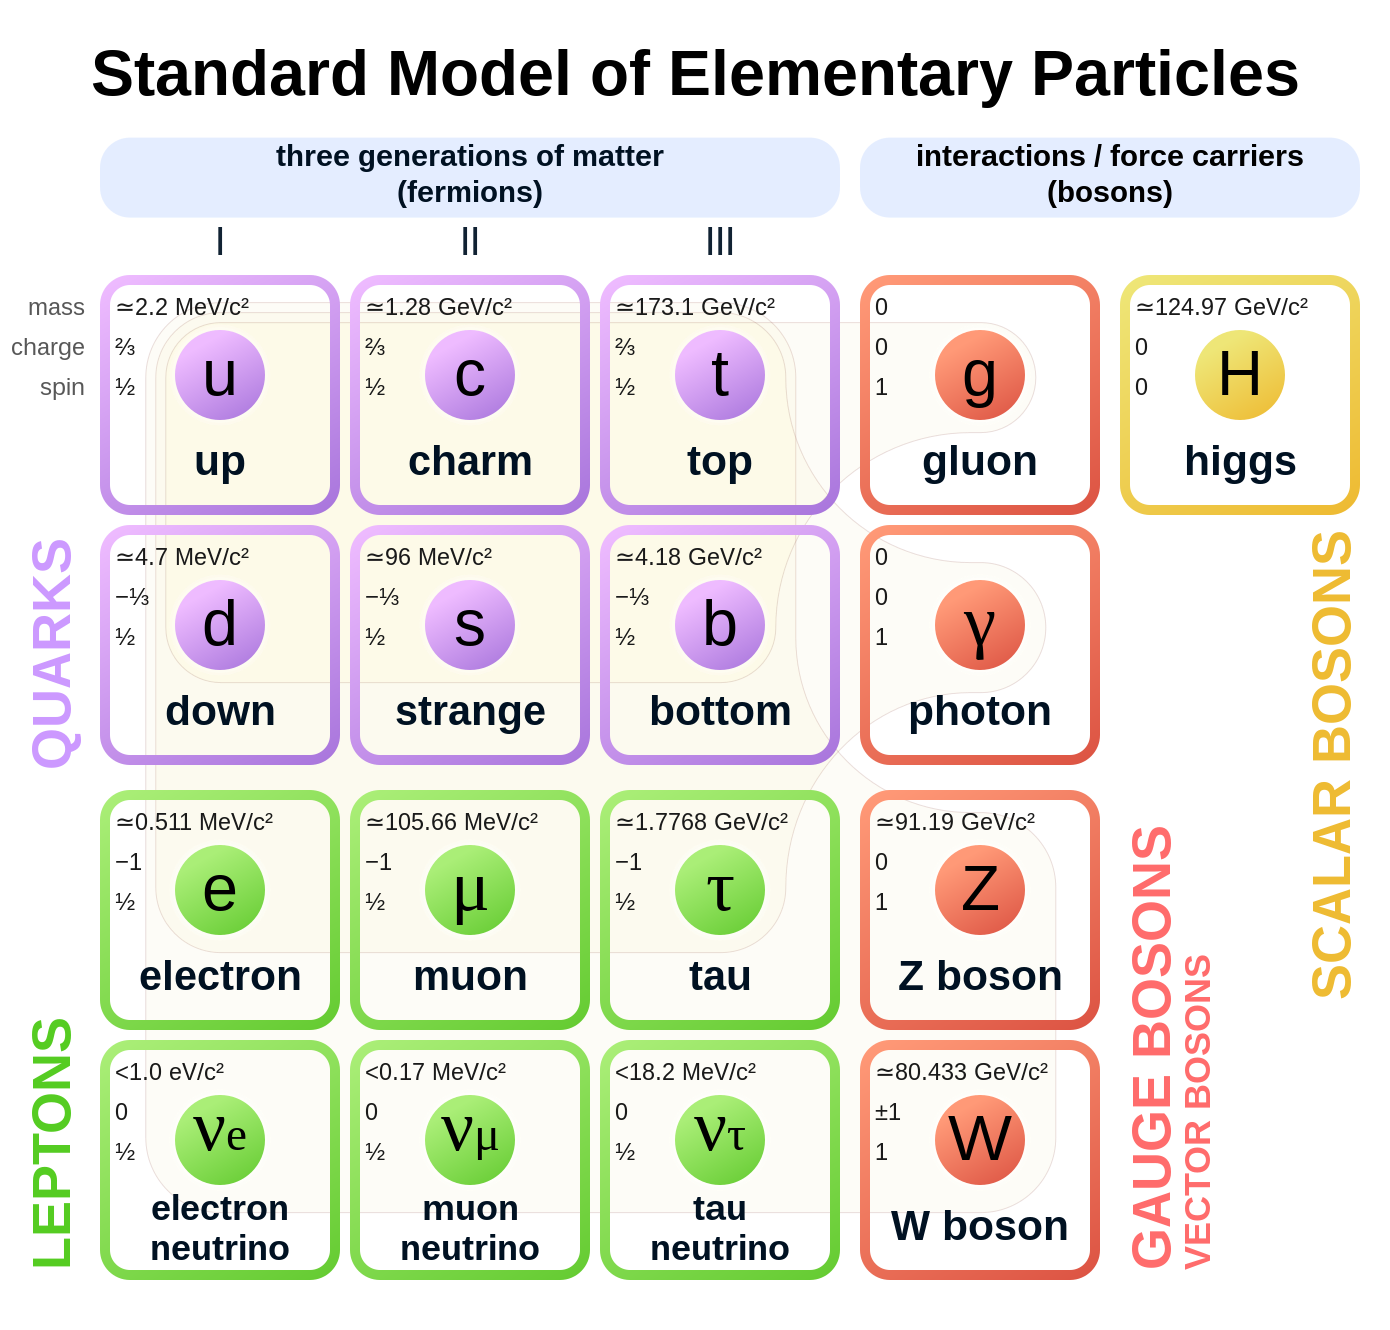
\includegraphics[width=\textwidth]{Figs/Chapter2/Standard_Model_of_Elementary_Particles.svg.png}\label{fig:StdModel}
	\caption{Classification of the elementary particles of the Standard Model, with the fermions on the left and the bosons (gauge and scalar) on the right. Figure taken from \cite{missmjStandardModelElementary2019}.}
	\label{fig:StdModel}
\end{figure}

Classically, a particle interacts with another through a field (for example, in electromagnetism, a positively charged particle generates an electric field that exerts an attractive/repulsive force on neighboring negative/positive charge). In QFT, fields are quantized, and the energy and momentum previously carried by the field are now conveyed by chunks, by quanta\footnote{Here, we present elementary particles as quanta  of their underlying field as if the particles could be reduced from their field, which corresponds to the usual experimentalist's picture of QFT. In fact, the relation between particles and fields is slightly more subtle \cite{jaegerElementaryParticlesQuantum2021}.} \cite{serwayModernPhysics2004}. So in particle physics, interactions are described as an exchange of quanta or spin-1 force-carrying particles, known as \textit{(vector) gauge bosons}\footnote{They are called \textit{bosons} because, contrarly to the fermions, their intrinsic angular momentum (or spin) has an integer value.}\cite{braibantParticlesFundamentalInteractions2012}\cite{thomsonModernParticlePhysics2013}. Following the remarks in \Sec\ref{subsec:Theory}, the term "(\textit{vector}) \textit{gauge}" emphasizes here the fact that the boson arises from a gauge vector field and thereby a gauge symmetry. 

The most successful quantum field theory is the quantum electrodynamics (QED) that describes the interaction between charged particles and electromagnetic fields. It has been developped between 1947 and 1949 by Shin'-ichir$\bar{\text{o}}$ Tomonaga, Julian Schwinger, Richard P. Feynman and Freeman Dyson; only the first three received the 1965 Nobel Prize in Physics for their contributions\footnote{Unfortunately F. Dyson did not receive the Nobel Prize because i) his work was not considered as groundbreaking as the one of the three other laureates and ii) the Nobel Prize in a given field can only be awarded to organisation of maximum of three individuals \cite{schmidhuberEvolutionNationalNobel2010}.}. It is based on a U(1) local gauge symmetry\footnote{U(N) corresponds to the group of all unitary matrices to size $N \times N$. Thus, U(1) is a group containing all the continuous transformation of the phase of a complex number.}, that results into an interaction with charged particles mediated by massless photons. This continuous symmetry is associated to a conserved quantity, namely the electric charge. The dynamics of this interaction is given by the Lagrangian density of QED in \eq\ref{eq:LagrangianQED}.

\begin{equation}
\Lagr_{QED} = \underbrace{i \bar{\psi} \gamma^{\mu} \partial_{\mu} \psi}_{\substack{\text{electron} \\ \text{kinetic term}}} + \underbrace{e \bar{\psi} \gamma^{\mu} A_{\mu} \psi}_{\substack{\text{electron-photon} \\ \text{interaction term}}} - \underbrace{m \bar{\psi} \psi}_{\substack{\text{electron} \\ \text{ mass term}}} - \underbrace{\frac{1}{4} F_{\mu \nu} F^{\mu \nu}}_{\substack{\text{photon} \\ \text{kinetic term}}} 
\label{eq:LagrangianQED}
\end{equation}
where
\begin{itemize}
\item[$\bullet$] $\gamma^{\mu}$ Dirac matrices that express the vectorial nature of the interaction and $\mu$ is the Lorentz vector index,
\item[$\bullet$] $A_{\mu}$ the photon field,
\item[$\bullet$] $F_{\mu \nu} = \partial_{\mu} A_{\nu} - \partial_{\nu} A_{\mu}$ the field-strength tensor,
\item[$\bullet$] $e$ the coupling constant of QED which coincides with the electric charge of the electron-positron field,
\item[$\bullet$] $m$ the electron/positron mass,
\item[$\bullet$] $\psi$ the electron-positron spinor field,
\end{itemize}
with the Einstein's notation $x^{\mu} x_{\mu} = \sum_{\mu=0}^{N} x^{\mu} x_{\mu}$ and the notations from \cite{thomsonModernParticlePhysics2013}.\\

\begin{figure}
\begin{center}
\unitlength = 1mm
\begin{fmffile}{eegamma}
\begin{fmfgraph*}(40,25)
\fmfleft{i1,i2}
\fmfright{o1}
\fmflabel{$e^-$}{i1}
\fmflabel{$e^+$}{i2}
\fmf{fermion}{i1,v1}
\fmf{fermion}{i2,v1}
\fmf{photon,label=$\gamma$}{v1,o1}
\end{fmfgraph*}
\end{fmffile}
\end{center}
\caption{Interaction vertex in QED. }
\end{figure}



Being the first quantum field theory developed, QED paved the way -- and even served as a template -- for all the subsequent quantum field theories. Therefore, it is not surprising that the form of Lagrangian density is the same for all the forces. 

Attempts to develop a quantum field theory for the weak interaction started in the 1950s, following the success of QED; none of them could provide satisfactory description. In the same decade, important discoveries have been made: the Wu's\footnote{Awarded of the 1957 Nobel Prize.} (1956) and Goldhaber's (1957) experiments \cite{wuExperimentalTestParity1957}\cite{goldhaberHelicityNeutrinos1958} showed that the P- and CP-symmetries are violated by the weak interaction. These led to conclude that this force has a vector-axial vector structure, meaning that only interacts with left-handed chiral particles and right-handed chiral anti-particles. Meanwhile, a few physicists -- including Schwinger, his PhD students Sheldon L. Glashow, Abdus Salam and Steven Weinberg -- foresaw that the weak and electromagnetic forces might be two aspects of the same phenomenon. Thanks to the work of Chen Ning Yang and Robert Mills on the development of a generalized gauge theory in 1954, Glashow delivered the electroweak interaction in 1961, which was consolidated later in 1967 and 1968 by Weinberg and Salam\footnote{For their contribution, Glashow, Salam and Weinberg receive the 1979 Nobel Prize.} respectively. In this quantum field theory, the electromagnetic and weak forces are described within an unified framework; the weak interaction is based on the SU(2) gauge group\footnote{The S (for "special") refers to the group of all matrices whose determinant is equal to 1.}, three generators hence three gauge bosons: \rmWplus, \rmWminus and \rmZzero. These bosons exhibit two unique properties.  First, contrarly to all other gauge bosons, these ones have an enormous mass (m$_{\rmWplusminus}$ = 80.377 \gmass and m$_{\rmZzero}$ = 91.1876 \gmass \cite{particledatagroup2022}), which explains why the weak force is such a short-range interaction. Second, the \rmWplusminus bosons can change the flavour of quarks and leptons. The trend (or the probability) of the flavour-changing is given by the \textbf{C}abibbo-\textbf{K}obayashi-\textbf{M}askawa\footnote{The Universe is unfair: similarly to Dyson for the QED, Nicolas Cabibbo (the pioneer of the CKM matrix) was not awarded with the 2008 Nobel Prize, while Makoto Kobayashi and Toshihide Maskawa were.} (CKM) matrix \cite{particledatagroupReviewParticlePhysics2022}\footnote{Mathematically speaking, this matrix relates the mass eigenstates to the weak eigentstates \cite{thomsonModernParticlePhysics2013}.} in \eq\ref{eq:CKMmatrix}.

\begin{equation}
V_{\textrm{CKM}} = 
\begin{pmatrix}
V_{\rm ud} & V_{\rm us} & V_{\rm ub}\\
V_{\rm cd} & V_{\rm cs} & V_{\rm cb}\\
V_{\rm td} & V_{\rm ts} & V_{\rm tb}
\end{pmatrix} = 
\begin{pmatrix}
0.97425 \pm 0.00022 & 0.2253 \pm 0.0008 & 0.00413 \pm 0.00049\\
0.225 \pm 0.008 & 0.986 \pm 0.016 & 0.0411 \pm 0.0013\\
0.0084 \pm 0.0006 & 0.040 \pm 0.0027 & 1.021 \pm 0.032
\end{pmatrix}\label{eq:CKMmatrix}
\end{equation}

Each matrix element provides the probability of transition from one flavour $i$ to another $j$ for quarks, but the same exists for the leptons and is called the \textbf{P}ontecorvo-\textbf{M}aki-\textbf{N}akagawa-\textbf{S}akata (PMNS) matrix. The elements of the PMNS matrix are slightly different from the CKM ones, the structure and ordering are the same, though. 

Finally, concerning the strong interaction, we will see later in its dedicated \Sec\ref{subsec:strongforce}. Patience!
\\


The overall picture of the Standard Model's elementary particles is presented in \fig\ref{fig:StdModel}. To this figure should be added the antiparticles. Indeed, to each particle -- fermion or boson --, there corresponds an antiparticle that have the same properties, because of the CPT invariance, but with oppositely sign quantum numbers. Consequently, this also means that both CKM and PMNS matrices are the same for particles and antiparticles.

There is, however, one element of the table in the \fig\ref{fig:StdModel} that has not been discussed yet, that is the Higgs boson. It originates from the electroweak unification, so let us retrace our steps. The principles of gauge invariance inevitably give rise to massless gauge bosons, like the photons but not the massive \rmWplusminus, \rmZzero bosons. At the time of Glashow's electroweak model in 1961, no one could imagine a mechanism to generate the enormous masses of the weak interaction force-carriers. In the same year, Jeffrey Goldstone showed that spontaneous symmetry breaking\footnote{This is the phenomenon in which a physical system perfectly symmetric breaks the symmetry without any external intervention. The most famous example of such process concerns the magnets. A material can be seen as an ensemble of microscopic magnets. If this material is ferromagnetic, all these magnets will tend to align with their neighbors.  When the temperature increases, the thermal motions start to disrupt this alignement until the material is not magnetized anymore. Conversely, as the material cools down, neighboring magnets starts to align until a critical temperature, when all the magnets lines up in one macroscopic direction. All directions are equivalent but the magnet has to choose one. This choice breaks the symmetic situation when all the directions are equivalent; that is a \textit{symmetry breaking}. Moreover, this choice is not influenced by any external agent, hence it is labelled as \textit{spontaneous}.} leads to the existence of massless gauge bosons, called Goldstone bosons. Three years later, in 1964, three independent groups (Robert Brout and François Englert; Peter Higgs; Gerald Guralnik, Carl Richard Hagen, and Tom Kibble) demonstrated the Goldstone bosons could be absorbed by the massless gauge bosons to acquire a mass: this is the Higgs mechanism. It is only in 1967-68, that Weinberg and Salam put to use this mechanism within Glashow's model to generate the masses of \rmWplusminus and \rmZzero bosons. But this goes beyond the scope of the electroweak unification; through this process is generated the mass of all elementary particles \cite{s.glashowInteractionsJourneyMind1990}. Incidentally, a new massive spinless particle, associated to a scalar field, is introduced out of the Higgs mechanism: the Higgs boson. Its observation in laboratory was at the heart of Standard Model research for decades until the 8th of October 2013 when the ATLAS and CMS experiments at the LHC at CERN announced the discovery of the Higgs boson. The same year, Peter Higgs and François Englert receive the Nobel Prize for their contribution to the Standard Model.


\subsection{The strong force, a colourful interaction}
\label{subsec:strongforce}

Back in the 1960s, in the "glorious years" of elementary particle physics, when physicists were submerged by the number of newly discovered "elementary" particles. Some of them were subject to the strong interaction, some were not; the former were refered as \textit{hadrons}\footnote{The expression originates from the Greek \textit{adros} meaning "thick and bulky".} and the latter as \textit{leptons}, as discussed in \Sec\ref{subsec:ParticleAndInteractions}. The hadrons were further sorted into two groups known as \textit{mesons} and \textit{baryons}\footnote{These terms originally refer to the mass of the particle: \textit{meson} comes from the Greek root \textit{meso} for "middle", that is in between the electron and proton masses; \textit{baryon} stem from Greek \textit{barys} for "heavy", suggesting any particle with a mass greater or similar to the one of the nucleons. Before the development of the quark model, the difference between the meson and the baryon was driven by their spin. The meson is a boson (integer spin values) where as the baryon is a fermion (half-integer spin values)\cite{s.glashowInteractionsJourneyMind1990}.}. But no one could draw out the underlying scheme between these particles and organise them into some kind of periodic table. There were some attempts though \cite{sakataCompositeModelNew1956}\cite{sakuraiTheoryStrongInteractions1960}; however the Mendeleev of particle physics is arguably Murray Gell-Mann. 

In 1961, he (and independently Yuval Ne'eman) proposed a classification scheme called the \textit{eightfold way} \cite{gell-mannEIGHTFOLDWAYTHEORY1961}\cite{neemanDerivationStrongInteractions1961}. At that time, eight spinless mesons, eight vector mesons with spin one and eight spin-half baryons were known. In each of these octets, a pattern emerges when the hadrons are organized into groups/multiplets of roughly the same mass, a hint of the underlying structure of strong interaction. A year later, the eightfold way is updated and completed with a decuplet formed of spin-$\frac{3}{2}$ baryons. However, one of the ten members of the decuplet was not yet discovered but this periodic table of elementary particles can predict its properties: a mass near the 1675 \mmass, strangeness\footnote{A quantum number introduced by Murray Gell-Mann in 1953 order to explain the \textit{strange} behaviour of some particles, such as kaons \cite{gell-mannIsotopicSpinNew1953}. Any particle with a non-zero strangeness value is dubbed \textit{strange particle}.} of -3 and negatively charged, this is the \rmOmegaM. Its existence is confirmed experimentally in 1964 by the Alternating Gradient Synchrotron at the Brookhaven National Laboratory (BNL)\cite{barnesObservationHyperonStrangeness1964a}, validating the eightfold way once and for all.\\

Within the year of this discovery, Murray Gell-Mann (and independently Georges Zweig) unveiled the symmetry behind the eightfold way: there are no elementary hadrons, they are, in fact, all built out of more fundamental particles named \textit{quarks}. A composite object made of bosons can only lead to a boson whereas, formed by fermions, the object is either a fermion or a boson depending on the number of constituents involved. Hence, the quarks must be fermions of spin one-half, mesons are composed of an even number of quarks, baryons of an odd number. The smallest odd number is one, but i) it does not make sense to say that a composite structure is made of one constituent and ii) we will see later in \Sec\ref{subsubsec:confinement} that a system of one quark is physically impossible. Thus, mesons must be made out of two quarks and baryons out of three; these are the simplest imaginable arrangements. 

Originally, quarks exist in two flavours, \textit{up} ($u$) and \textit{down} ($d$), with fractional electric charges of $+2e/3$ and $-1e/3$ respectively. An extra flavour was needed to explain the existence of strange hadrons: the strange quark, $s$, is born. It has the same properties as the $d$-quark, except that it is much heavier and it has an assigned strangeness number of -1. Any strange hadrons actually contains one to three $s$-quark, depending on their strangeness. Therefore, the predicted particle by the eightfold way, the \rmOmegaM, corresponds actually to the strangest hadron possible, a baryon with three strange quarks. 

With this particle comes the first difficulty of the quark model. Whatever the particle, it must obey the spin-statistics theorem. Quarks being fermions, the theorem states that two \textit{identical} fermions can not occupy the same quantum states simultaneously. However, \rmOmegaM is constituted of three exactly identical $s$-quark \cite{skandsIntroductionQCD2013}. This problem was overcome by Oscar W. Greenberg \cite{greenbergSpinUnitarySpinIndependence1964}, Moo-Young Han and Yoichiro Nambu \cite{hanThreeTripletModelDouble1965} in 1964-65 that introduced a new quantum number, the colour. Each quark comes in three colours or variants labelled as red ($r$), green ($g$) and blue ($b$). In this way, the spin-statistics problem is solved but new questions arises. If quarks carry a colour, hadrons are a mixture of colours. This is assumed to be an equal mixture of all the colours, such that the hadrons are colourless. How come? Why are there no colour hadrons? 

Along the same line: in 1966, the main accelerator at the Stanford Linear Accelerator Center (SLAC) becomes operational and starts a program of deep inelastic scattering experiments in order to study the inner structure of nucleons. Based on James Bjorken \cite{bjorkenCurrentAlgebraSmall2018} and Richard Feynman  \cite{feynmanBehaviorHadronCollisions1988} calculations, the results of SLAC's experiments, in 1969, showed that the nucleons were made of point-like constituents of spin-$\frac{1}{2}$, dubbed \textit{partons}, behaving as free particles \cite{peskinIntroductionQuantumField2018}. The partons were nothing else than the quarks, and these observations established the validity the quark picture to the whole particle physics community. However, it is curious that the partons seem to behave as free particles but they can not escape the hadron.\\

These questions remain unanswered until 1973. This year had seen the development of Quantum Chromodynamics (QCD) -- the quantum field theory of the strong force -- and the discovery of two of its most salient properties, namely the colour confinement and the asymptotic freedom (discussed in \Sec\ref{subsubsec:confinement} and \ref{subsubsec:asymptotic freedom}). Fruit of the work of Harald Fritzsch, Heinrich Leutwyler and Murray Gell-Mann \cite{fritzschAdvantagesColorOctet1973}, the QCD describes the interaction between colour-charged objects, namely the partons. It is based on the gauge symmetry group SU(3), which has eight generators, giving rise to eight massless gauge bosons called \textit{gluons}, and imposes the conservation of colour. 

QCD is very similar to QED: the electric charge is replaced by a colour charge, antiparticles carry opposite colour charges, and the eight gluons take the role of the photon. The dynamics of QCD is given by the Lagrangian density in \eq\ref{eq:LagrangianQCD}.\\

\begin{equation}
\Lagr_{QCD} = \underbrace{i \bar{\psi}_{q}^{i} \gamma^{\mu} \delta_{ij} \partial_{\mu} \psi_{q}^{j}}_{\substack{\text{quark} \\ \text{kinetic term}}} + \underbrace{g_{s} \bar{\psi}_{q}^{i} \gamma^{\mu} t_{ij}^{a} A_{\mu}^{a} \psi_{q}^{j}}_{\substack{\text{quark-gluon} \\ \text{interaction term}}} - \underbrace{m_{q} \bar{\psi}_{q}^{i} \psi_{qi}}_{\substack{\text{quark} \\ \text{mass term}}} - \underbrace{\frac{1}{4} F_{\mu \nu}^{a} F^{a \mu \nu}}_{\substack{\text{gluon} \\ \text{kinetic term}}} 
\label{eq:LagrangianQCD}
\end{equation}
where, using the notations from \cite{skandsIntroductionQCD2013},
\begin{itemize}
\item[$\bullet$] $g_s^2 = 4 \pi \alpha_s$ with $\alpha_{s}$ the coupling constant of QCD,
\item[$\bullet$] $F_{\mu \nu}^{a} = \underbrace{\partial_{\mu} A_{\nu}^{a} - \partial_{\nu} A_{\mu}^{a}}_{\text{Abelian}} + \underbrace{g_{s} f^{abc} A_{\mu}^{b} A_{\nu}^{c}}_{\text{non-Abelian}}$ the field-strength tensor,
\item[$\bullet$] $\psi_{q}^{i}$ the quark field spinor with colour index $i$ such that $\psi_{q} = \left({\color{red}\psi_{qR}}, {\color{green}\psi_{qG}}, {\color{blue}\psi_{qB}} \right)^{\rm T} $,
\item[$\bullet$] $m_{q}$ the quark \textit{bare} mass induced by the Higgs mechanism,
\item[$\bullet$] $A_{\mu}^{a}$ the gluon field with colour index $a$,
\item[$\bullet$] $t_{ij}^{a} = \frac{1}{2} \lambda_{ij}^{a}$ and $\lambda^{a}$ the fundamental\footnote{The representation of a group is \textit{fundamental} when its generators are hermitian and traceless matrices. } representation of the generator of SU(3) associated to the colour index $a$,
\item[$\bullet$] $f^{abc}$ the structure constants of SU(3).\\
\end{itemize}

As in QED, the Lagrangian density can be expressed with four terms; the quark-gluon interaction is described by the second one. However, the field-strength tensor $F_{\mu \nu}^{a}$ here admits an extra term because the generators of SU(3) do not commute. The non-Abelian property of the gauge group of QCD gives rise to gluon-self interactions, as shown in the Feynman's diagrams of \fig\ref{fig:FeynmanDiagQCD}.

\begin{figure}[h]
\begin{center}
\unitlength = 1mm
\subfigure[]{
	\begin{fmffile}{qqg}
	\begin{fmfgraph*}(40,25)
	\fmfleft{i1,i2}
	\fmfright{o1}
	\fmflabel{$q$}{i1}
	\fmflabel{$\bar{q}$}{i2}
	\fmf{fermion}{i1,v1}
	\fmf{fermion}{v1,i2}
	\fmf{gluon,label=$g$, lab.dist=0.1w}{v1,o1}
	\end{fmfgraph*}
	\end{fmffile}
}
\subfigure[]{
	\begin{fmffile}{ggg}
	\begin{fmfgraph*}(40,25)
	\fmfleft{i1,i2}
	\fmfright{o1}
	\fmflabel{$g$}{i1}
	\fmflabel{$g$}{i2}
	\fmflabel{$g$}{o1}
	\fmf{gluon}{i1,v1}
	\fmf{gluon}{i2,v1}
	\fmf{gluon}{v1,o1}
	\fmfv{lab=$g_s$,lab.dist=0.15w}{v1}
	\fmfdot{v1}
	\end{fmfgraph*}
	\end{fmffile}
}
\subfigure[]{
	\begin{fmffile}{gggg}
	\begin{fmfgraph*}(40,25)
	\fmfleft{i1,i2}
	\fmfright{o1,o2}
	\fmflabel{$g$}{i1}
	\fmflabel{$g$}{i2}
	\fmflabel{$g$}{o1}
	\fmflabel{$g$}{o2}
	\fmf{gluon}{i1,v1}
	\fmf{gluon}{i2,v1}
	\fmf{gluon}{v1,o1}
	\fmf{gluon}{v1,o2}
	\fmfv{lab=$g_s^2$,lab.dist=0.15w}{v1}
	\fmfdot{v1}
	\end{fmfgraph*}
	\end{fmffile}
}
\end{center}
\caption{The three possible interaction vertices within the framework of QCD: (a) quark-gluon, (b) triple-gluon and (c) four-gluon interactions.}
\label{fig:FeynmanDiagQCD}
\end{figure}

There are several consequences to the self-interaction of gluons.

\begin{figure}[h]
	\centering
	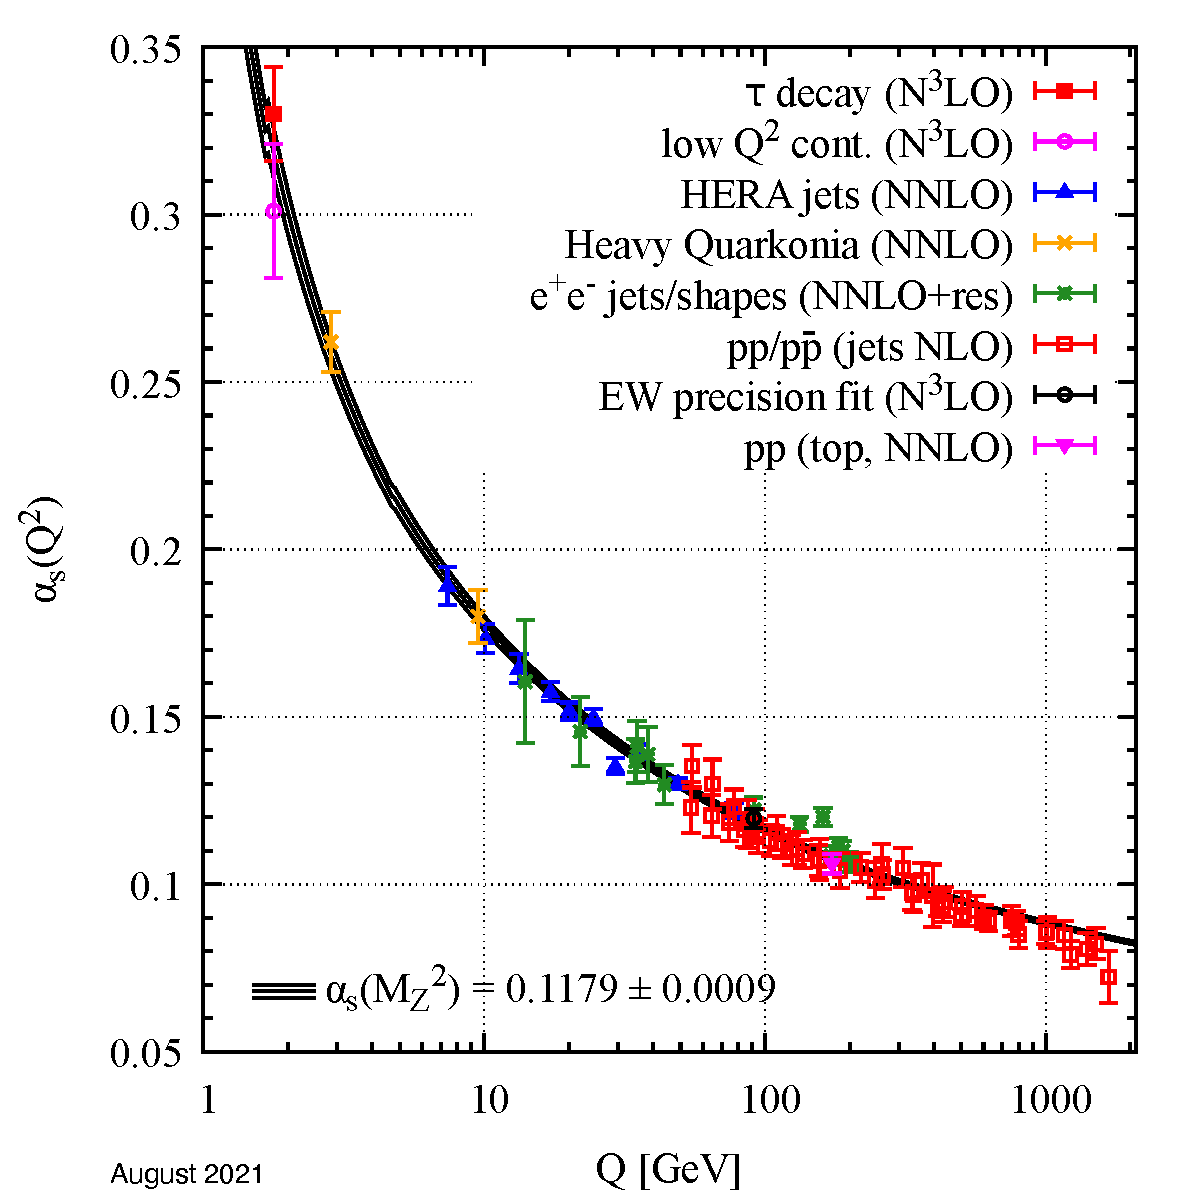
\includegraphics[width=0.8\textwidth]{Figs/Chapter2/alphas-v-Q-2021.pdf}
	\caption{Classification of the elementary particles of the Standard Model, with the fermions on the left and the bosons (gauge and scalar) on the right. Figure taken from \cite{deurQCDRunningCoupling2016}.}
	\label{fig:RunningAlphaS}
\end{figure}

\begin{figure}[h]
	\centering
	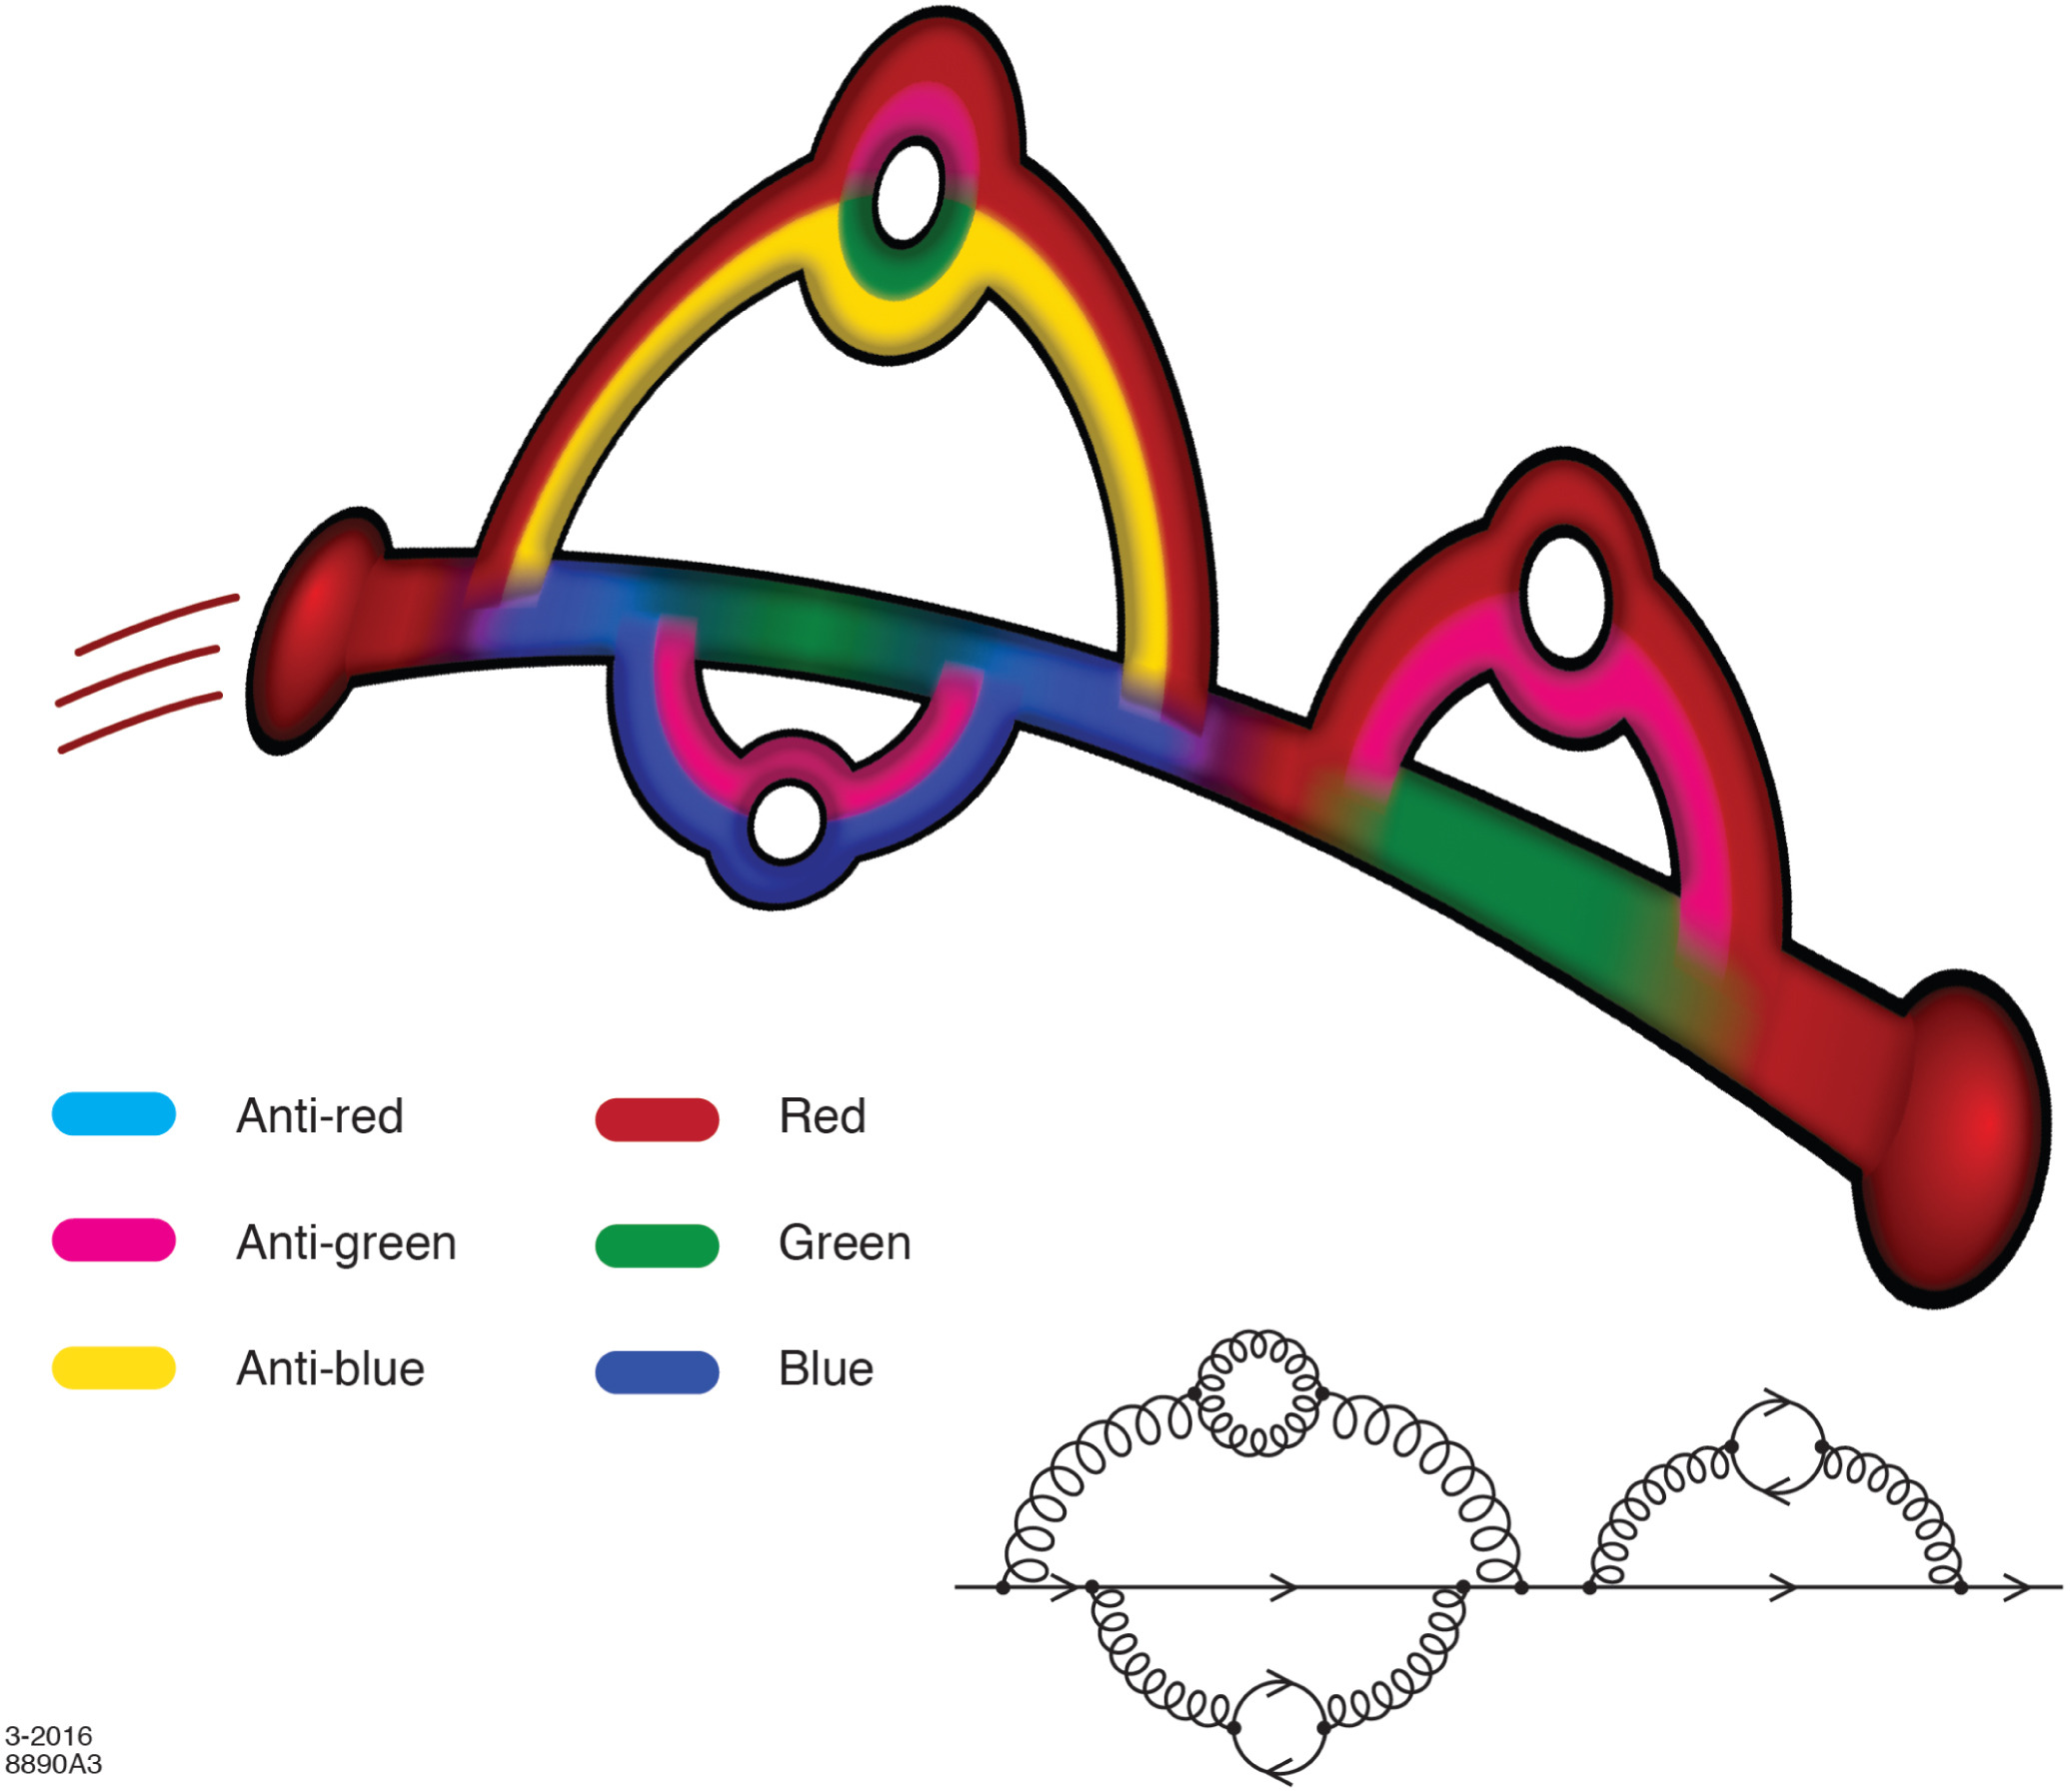
\includegraphics[width=0.8\textwidth]{Figs/Chapter2/1-s2.0-S0146641016300035-gr1_lrg.jpg}
	\caption{Classification of the elementary particles of the Standard Model, with the fermions on the left and the bosons (gauge and scalar) on the right. Figure taken from \cite{deurQCDRunningCoupling2016}.}
	\label{fig:ColourSpread}
\end{figure}

\subsubsection{Colour confinement}
\label{subsubsec:confinement}


Confinement scale $\Lambda_{QCD} \sim 400 MeV$

$m_{t}, m_{b} m_{c} \gg \Lambda_{QCD} \gg m_{s}, m_{u}, m_{d}$
--> allows to define heavy and light sector

\subsubsection{Asymptotic freedom}
\label{subsubsec:asymptotic freedom}

\cite{grossUltravioletBehaviorNonAbelian1973} \cite{davidpolitzerAsymptoticFreedomApproach1974}

\subsubsection{Chiral symmetry breaking}
\label{subsubsec:chiralsymmetrybreaking}

\subsubsection{The QCD-phase diagram}
\label{subsubsec:QCDphasediagram}

\section{Experimental signatures of the QGP}

\subsection{The time evolution of a Heavy-Ion collision}

\begin{figure}[h]
	\centering
	\includegraphics[width=\textwidth]{Figs/Chapter2/QGP_Evol.eps}
	\caption{Classification of the elementary particles of the Standard Model, with the fermions on the left and the bosons (gauge and scalar) on the right. Figure taken from \cite{missmjStandardModelElementary2019}.}
	\label{fig:QGPEvol}
\end{figure}

\subsection{Strangeness enhancement}

\begin{figure}[h]
	\centering
	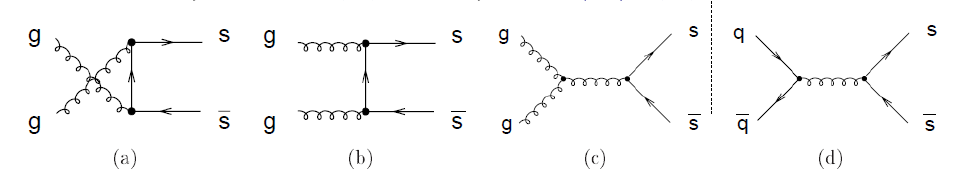
\includegraphics[width=\textwidth]{Figs/Chapter2/Screenshot_20220620_004959.png}
	\caption{Classification of the elementary particles of the Standard Model, with the fermions on the left and the bosons (gauge and scalar) on the right. Figure taken from \cite{missmjStandardModelElementary2019}.}
	\label{fig:StrangenessEnhancement}
\end{figure}

%\begin{figure}
%\unitlength = 1mm
%\centering
%\subfigure[]{
%	\begin{fmffile}{ggxss}
%	\begin{fmfgraph*}(40,25)
%	\fmfleft{i1,i2}
%	\fmfright{o1,o2}
%	\fmflabel{$g$}{i1}
%	\fmflabel{$g$}{i2}
%%	\fmflabel{$s$}{o1}
%%	\fmflabel{$\bar{s}$}{o2}
% 	\fmf{fermion}{o1,v1}
% 	\fmf{fermion,tension=0}{v1,v2}
% 	\fmf{fermion}{v2,o2}
% 	\fmffreeze
%	\fmf{gluon}{i1,v2}
%	\fmf{gluon,rubout}{i2,v1}
%%    \fmf{fermion}{i1,v1,v2,o1}
%%	\fmf{fermion}{o2,v4,v3,i2}
%%	\fmf{photon,tension=0}{v1,v3}
%%	\fmf{photon,tension=0}{v2,v4}
%	\end{fmfgraph*}
%	\end{fmffile}
%}
%\subfigure[]{
%	\begin{fmffile}{gghss}
%	\begin{fmfgraph*}(40,25)
%	\fmfleft{i1,i2}
%	\fmfright{o1}
%	\fmflabel{$g$}{i1}
%	\fmflabel{$g$}{i2}
%	\fmflabel{$g$}{o1}
%	\fmf{gluon}{i1,v1}
%	\fmf{gluon}{i2,v1}
%	\fmf{gluon}{v1,o1}
%	\fmfv{lab=$g_s$,lab.dist=0.15w}{v1}
%	\fmfdot{v1}
%	\end{fmfgraph*}
%	\end{fmffile}
%}
%\subfigure[]{
%	\begin{fmffile}{ggss}
%	\begin{fmfgraph*}(40,25)
%	\fmfleft{i1,i2}
%	\fmfright{o1,o2}
%	\fmflabel{$g$}{i1}
%	\fmflabel{$g$}{i2}
%	\fmflabel{$g$}{o1}
%	\fmflabel{$g$}{o2}
%	\fmf{gluon}{i1,v1}
%	\fmf{gluon}{i2,v1}
%	\fmf{gluon}{v1,o1}
%	\fmf{gluon}{v1,o2}
%	\fmfv{lab=$g_s^2$,lab.dist=0.15w}{v1}
%	\fmfdot{v1}
%	\end{fmfgraph*}
%	\end{fmffile}
%}
%\subfigure[]{
%	\begin{fmffile}{qqss}
%	\begin{fmfgraph*}(40,25)
%	\fmfleft{i1,i2}
%	\fmfright{o1,o2}
%	\fmflabel{$g$}{i1}
%	\fmflabel{$g$}{i2}
%	\fmflabel{$g$}{o1}
%	\fmflabel{$g$}{o2}
%	\fmf{gluon}{i1,v1}
%	\fmf{gluon}{i2,v1}
%	\fmf{gluon}{v1,o1}
%	\fmf{gluon}{v1,o2}
%	\fmfv{lab=$g_s^2$,lab.dist=0.15w}{v1}
%	\fmfdot{v1}
%	\end{fmfgraph*}
%	\end{fmffile}
%}
%\caption{Using \texttt{test}}
%\end{figure}

\subsection{Comparison with elementary systems}


    



